\documentclass{article}
% Numeric citations (NeurIPS standard): pass options before neurips loads natbib.
\PassOptionsToPackage{numbers,sort&compress}{natbib}
\usepackage{neurips_2026}
\usepackage[utf8]{inputenc}
\usepackage[T1]{fontenc}
\usepackage{hyperref}
\usepackage{url}
\usepackage{booktabs}
\usepackage{amsfonts}
\usepackage{amsmath}
\usepackage{amssymb}
\usepackage{microtype}
\usepackage{xcolor}
\usepackage{graphicx}
\usepackage{caption}
\usepackage{tikz}
\usetikzlibrary{arrows.meta,positioning,fit,calc}
\usepackage{placeins}

\title{CALM: A Unified v1--v2 Framework for Reliable Few-Shot and Continual Vision\\with Confidence-Aware Deployment}

\author{Anonymous Authors}

\begin{document}
\maketitle

\begin{abstract}
We introduce CALM (Continual Adaptive Learning Model) for few-shot and continual vision with confidence-aware deployment. CALM-v1 combines a frozen vision-language backbone, episodic memory, prototypical classification, and a readiness agent; CALM-v2 extends this design with multi-encoder confidence signals and hierarchical compressed memory. Under protocol-matched ImageNet evaluations (5-way 5-shot episodic learning with 600 episodes; 10-task continual learning with 5-shot memory), we compare both versions to commonly reported baselines and to each other. In our setting, CALM-v1 reaches $96.88\%$ few-shot accuracy and $-5.52\%$ backward transfer (BWT), while CALM-v2 (ensemble) attains $96.16\% \pm 0.32\%$ and $-5.97\%$ BWT at temperature $T=1.0$. We discuss how deployment-oriented changes in v2 may interact with prototype geometry, and we summarize practical recommendations---including a single-backbone ablation protocol---aimed at improving representation consistency. Together, the paper clarifies trade-offs between core task metrics and reliability-oriented design choices in non-parametric VLM adaptation.
\end{abstract}

\section{Introduction}
Foundation vision-language models (VLMs), such as CLIP~\citep{radford2021clip}, provide strong off-the-shelf representations, yet practitioners still face competing demands: adapting quickly from few labels, retaining performance as tasks arrive sequentially, and avoiding unsafe silent failures at deployment. Gradient fine-tuning and many parameter-efficient schemes remain costly or fragile under distribution shift; training-free or memory-based alternatives therefore attract growing interest.

CALM-v1 follows this line by keeping the VLM frozen, maintaining an episodic memory of embeddings, classifying with prototypical inference, and gating predictions with a temperature-calibrated readiness agent that can request human feedback. In our ImageNet experiments, that design reaches $96.88\%$ on 5-way 5-shot episodic evaluation and $-5.52\%$ BWT on a 10-task continual protocol, suggesting that non-parametric adaptation can be effective without backbone updates.

CALM-v2 explores a natural next step: richer confidence estimates from disagreement across two CLIP encoders, together with hierarchical memory that compresses older embeddings to stretch effective capacity. These changes are motivated by deployment settings where uncertainty quality and memory growth matter, but they also couple multiple representation spaces to shared prototypes in ways that are easy to underestimate during design.

\textbf{Scope and novelty.} CALM-v1 and CALM-v2 are both our contributions and, to the best of our knowledge, have not been published before. This submission presents them together: we (i) define CALM-v1 and its extension CALM-v2, (ii) evaluate both under identical ImageNet episodic and continual protocols alongside standard baselines, (iii) analyze where v2 differs from v1 in our measurements and discuss plausible mechanisms (with emphasis on cross-encoder consistency), and (iv) specify a single-backbone CALM-v2 ablation and reproducibility-oriented detail. The emphasis is on an integrated system---frozen VLM, episodic prototypes, calibrated deployment gating, and optional ensemble/hierarchical-memory extensions---rather than on any single isolated component.

\textbf{Contributions.}
\begin{itemize}
    \item We introduce CALM with two instantiations---CALM-v1 (frozen CLIP, episodic memory, prototypical classification, readiness agent) and CALM-v2 (multi-encoder confidence and hierarchical compressed memory)---and report ImageNet results under matched evaluation scripts and temperatures.
    \item Through implementation-level inspection and the observed metric shifts, we argue that cross-backbone prototype/query inconsistency is a \emph{plausible} and actionable explanation for part of the v2 gap relative to v1, rather than the only possible factor.
    \item We specify a single-backbone CALM-v2 ablation protocol that retains hierarchical memory but scores queries in one encoder space, to separate memory design from fusion effects.
    \item We report reproducibility-oriented protocol and evaluation detail in the main text suitable for NeurIPS-style reporting.
\end{itemize}

\section{Related Work}
\paragraph{Few-shot meta-learning and prototype methods.}
Prototypical Networks~\citep{snell2017proto} remain a reference for episodic few-shot learning but typically train task-specific encoders from scratch, which can be data-hungry and less aligned with modern frozen VLMs. Subsequent work shows that nearest-prototype or cache-style decision rules on top of frozen features can be surprisingly strong when the backbone is already semantic~\citep{radford2021clip,zhang2022tipadapter}. A recurring limitation of ``adapter-only'' methods, however, is that they seldom couple prediction with an explicit deployment policy: confidence is often treated as a by-product rather than a first-class control signal for abstention or human review.

\paragraph{Training-free CLIP adaptation.}
Tip-Adapter~\citep{zhang2022tipadapter} demonstrates competitive accuracy without fine-tuning the CLIP trunk, using a residual cache on embeddings. While effective for batch evaluation, it does not address continual task streams, memory budgets that grow without bound, or structured human-in-the-loop updates in the sense of CALM's readiness agent. CALM-v1 instead treats memory as the adaptation substrate and ties calibrated scores to deploy/request decisions~\citep{guo2017calibration}.

\paragraph{Continual learning with pre-trained models.}
Classical regularization approaches such as EWC~\citep{kirkpatrick2017ewc} mitigate forgetting but can underperform rehearsal when representations are fixed. iCaRL~\citep{rebuffi2017icarl} exemplifies exemplar-based continual learning with parametric classifiers; prompt-tuning methods including L2P~\citep{wang2022l2p} and DualPrompt~\citep{wang2022dualprompt} adapt internal activations for sequential tasks and can achieve high average accuracy, but at the cost of modifying the backbone pathway and a different computational profile than frozen-feature episodic systems. Recent empirical studies with foundation models reinforce that replay in feature space can be practical when drift is managed~\citep{hayes2024latentreplay}. CALM occupies a complementary niche: frozen encoders, explicit episodic storage, and non-parametric prototypes---useful when fine-tuning is disallowed or expensive, but not necessarily optimal on every continual metric relative to state-of-the-art prompt methods.

\paragraph{Calibration, conformal methods, and human oversight.}
Temperature scaling~\citep{guo2017calibration} remains a simple post-hoc calibration baseline. Distribution-free uncertainty tools such as conformal prediction~\citep{angelopoulos2021conformal} and multimodal extensions~\citep{chen2024conformalvlm} motivate separating coverage guarantees from raw softmax scores. Human-in-the-loop designs for large multimodal models similarly emphasize selective querying of users~\citep{zhang2024humanloop}. CALM-v1 instantiates a lightweight threshold policy; CALM-v2 explores richer signals (ensemble spread) while still aiming for deployable logic.

\paragraph{Memory scaling and hierarchical representations.}
Long-horizon systems must manage storage; hierarchical or compressed memory appears in large-scale vision-language stacks~\citep{deepseekocr2024,deepseekvl22024}. CALM-v2 adapts this idea to episodic embedding buffers so older examples occupy fewer bits, trading reconstruction error for capacity.

\paragraph{Position relative to prior work.}
The above lines of work are often evaluated in isolation: strong few-shot numbers without deployment policies, or continual methods that assume parametric heads and gradient access. CALM seeks an integrated story---frozen VLM, episodic prototypes, calibrated gating---and CALM-v2 stresses an under-discussed systems question: when multiple frozen encoders contribute to confidence and memory is lossy, \emph{which} similarities are computed in \emph{which} space? Our experiments and recommendations are aimed at that coupling.

\section{Method}\label{sec:method}

\subsection{Problem formulation}
We formalize the adaptive vision learning problem as follows. Given a pre-trained vision-language model with image encoder $f_\theta: \mathcal{X} \rightarrow \mathbb{R}^d$, where $\mathcal{X}$ is the input image space and $d$ is the embedding dimension, we adapt to a new task $\mathcal{T} = \{(\mathbf{x}_i, y_i)\}_{i=1}^{n}$ with $K$ classes while preserving the backbone's general knowledge.

The adaptation must satisfy three constraints:
\begin{align}
&\text{Efficiency: } \mathcal{O}(\text{adaptation}) \ll \mathcal{O}(\text{fine-tuning}) \label{eq:efficiency}\\
&\text{Preservation: } \|\theta_{\text{adapted}} - \theta_{\text{original}}\|_2 = 0 \label{eq:preservation}\\
&\text{Reliability: } P(\text{error}\mid\text{deploy}) \leq \epsilon \label{eq:reliability}
\end{align}
where $\epsilon$ is a user-defined error tolerance.

\subsection{CALM-v1}
CALM-v1 combines a frozen VLM backbone, dynamic episodic memory, prototypical classification, a readiness agent with temperature-scaled confidence, and human-in-the-loop memory updates. The following paragraphs state the v1 formulation we implement (notation and equations kept consistent throughout the paper).

\paragraph{Frozen VLM feature extractor.}
The foundation of CALM-v1 is a frozen vision-language model, specifically CLIP (ViT-B/32), employed as an immutable feature extractor:
\begin{equation}
\mathbf{e} = f_\theta(\mathbf{x}) \in \mathbb{R}^d
\end{equation}
where $\mathbf{x} \in \mathcal{X}$ is an input image and $\mathbf{e}$ is the corresponding $d$-dimensional embedding. The parameter freezing constraint $\nabla_\theta \mathcal{L} = 0$ ensures computational efficiency while preserving the rich semantic representations learned during pre-training.

\paragraph{Episodic memory and prototypical classification.}
Adaptation occurs through a dynamic episodic memory structure:
\begin{equation}
\mathcal{M} = \{(\mathbf{e}_i, y_i)\}_{i=1}^N
\end{equation}
where each tuple contains a feature embedding $\mathbf{e}_i \in \mathbb{R}^d$ and its corresponding class label $y_i \in \{1,2,\ldots,K\}$.

For classification, we compute class prototypes as centroids of support embeddings:
\begin{equation}
\mathbf{c}_k = \frac{1}{|S_k|} \sum_{(\mathbf{e}_i, y_i) \in S_k} \mathbf{e}_i \label{eq:prototype}
\end{equation}
where $S_k = \{(\mathbf{e}_i, y_i) \in \mathcal{M} \mid y_i = k\}$ denotes the support set for class $k$.

The classification probability distribution over classes is computed using cosine similarity-based softmax:
\begin{equation}
p(y=k\mid\mathbf{x}) = \frac{\exp(\cos(\mathbf{e}_x, \mathbf{c}_k) / \tau)}{\sum_{j=1}^{K} \exp(\cos(\mathbf{e}_x, \mathbf{c}_j) / \tau)} \label{eq:classification}
\end{equation}
where $\mathbf{e}_x = f_\theta(\mathbf{x})$ and $\tau$ is a temperature parameter for confidence calibration.

\paragraph{Readiness agent.}
The readiness agent $\mathcal{A}: \mathbb{R}^K \rightarrow \{0,1\}$ implements a two-stage decision process. \emph{Confidence calibration.} We employ temperature scaling to calibrate raw prediction confidences. The calibrated confidence score is:
\begin{equation}
q_x = \max_k \frac{\exp(\cos(\mathbf{e}_x, \mathbf{c}_k) / T)}{\sum_{j=1}^{K} \exp(\cos(\mathbf{e}_x, \mathbf{c}_j) / T)} \label{eq:calibration}
\end{equation}
where $T$ is the calibration temperature optimized by minimizing negative log-likelihood on a validation set:
\begin{equation}
T^* = \arg\min_T \sum_{i=1}^{n_{\text{val}}} -\log p(y_i\mid\mathbf{x}_i; T). \label{eq:temperature_opt}
\end{equation}

\emph{Decision logic.} The agent's binary decision function is defined as:
\begin{equation}
\mathcal{A}(q_x) = \begin{cases}
1 \text{ (Deploy)} & \text{if } q_x \geq \delta \\
0 \text{ (Request)} & \text{if } q_x < \delta
\end{cases} \label{eq:decision}
\end{equation}
The threshold $\delta$ is calibrated to achieve a target deployment rate $\rho$ by solving:
\begin{equation}
\delta^* = \arg\min_\delta \left|\frac{1}{n_{\text{val}}} \sum_{i=1}^{n_{\text{val}}} \mathcal{A}(q_i) - \rho\right|. \label{eq:threshold_opt}
\end{equation}

\paragraph{Human-in-the-loop learning.}
When the readiness agent requests feedback ($\mathcal{A}(q_x) = 0$), human experts provide correct labels $y_{\text{correct}}$. The system updates the episodic memory by appending the corrected tuple:
\begin{equation}
\mathcal{M} \leftarrow \mathcal{M} \cup \{(f_\theta(\mathbf{x}), y_{\text{correct}})\} \label{eq:memory_update}
\end{equation}
which immediately updates the relevant class prototype via Equation~\eqref{eq:prototype}, enabling real-time knowledge refinement without gradient-based optimization.

Figure~\ref{fig:v1_pipeline} summarizes the CALM-v1 pipeline.
\begin{center}
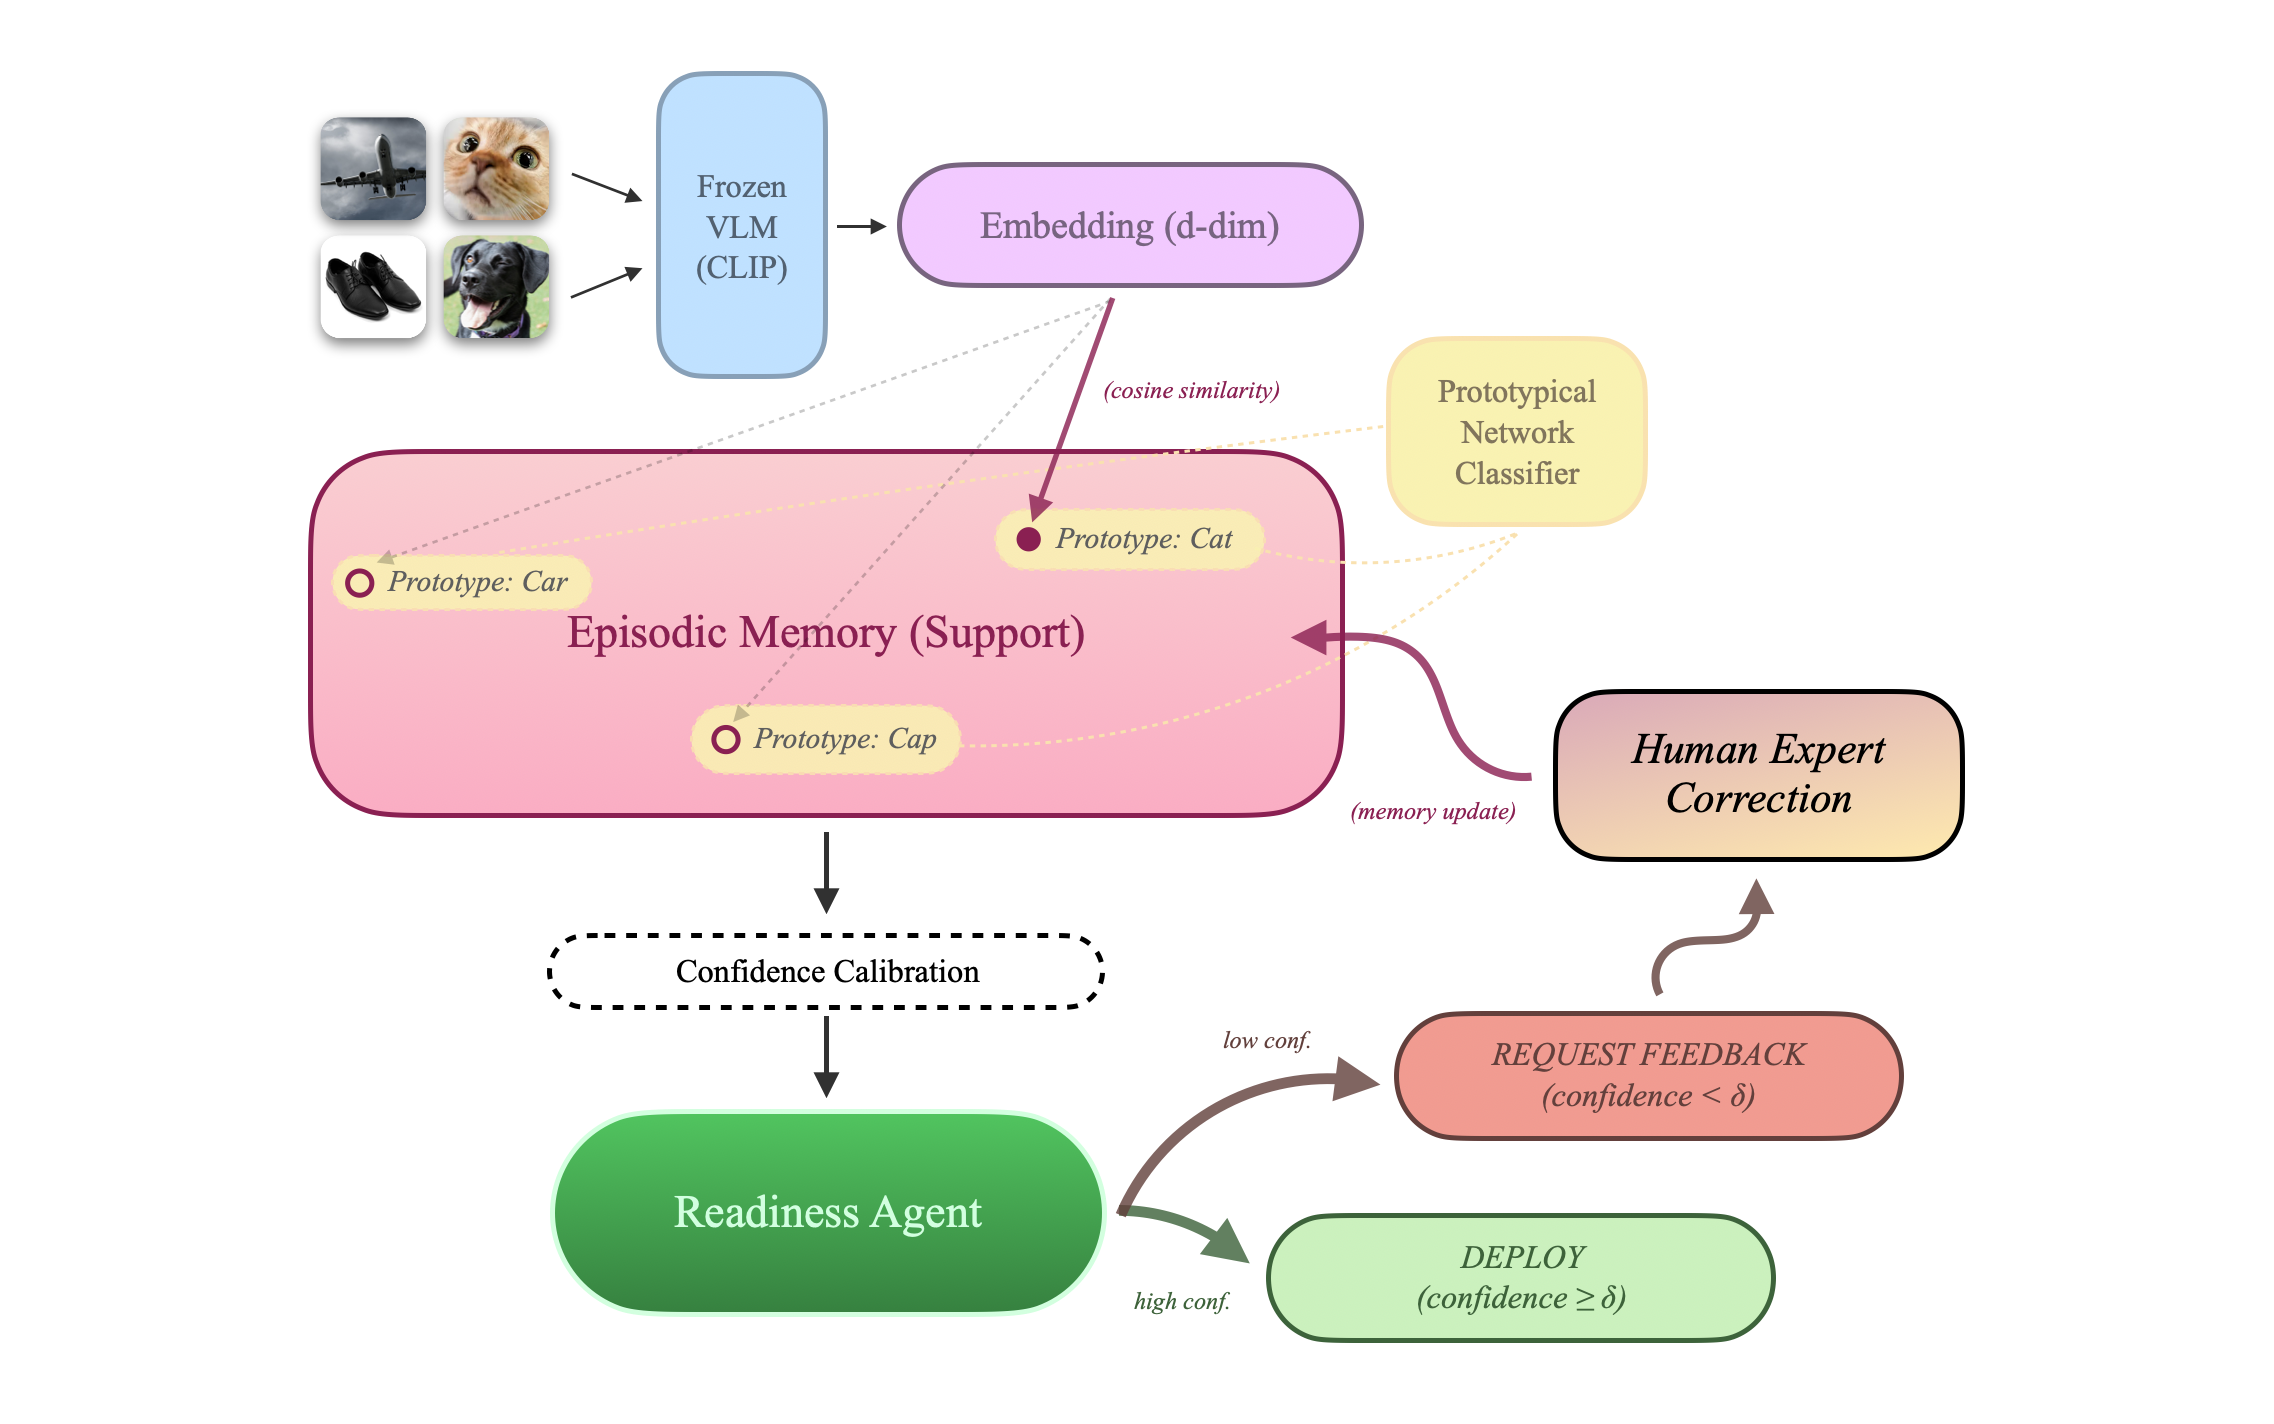
\includegraphics[width=\linewidth]{calm-v1.png}
\end{center}
\captionof{figure}{\textbf{CALM-v1 architecture and decision flow.} Input images are encoded by a frozen CLIP backbone $f_\theta:\mathcal{X}\to\mathbb{R}^d$ into $d$-dimensional embeddings while keeping pre-trained weights fixed. Embeddings are compared to class prototypes in episodic memory $\mathcal{M}=\{(\mathbf{e}_i,y_i)\}$ using cosine similarity within a prototypical-network classifier. Prediction scores undergo temperature-based calibration before a readiness agent $\mathcal{A}:\mathbb{R}^K\to\{0,1\}$ applies a threshold $\delta$ on confidence. High-confidence cases are deployed autonomously; uncertain cases request human labels and immediately update $\mathcal{M}$, yielding closed-loop non-parametric adaptation without backbone fine-tuning.}
\label{fig:v1_pipeline}

\subsection{CALM-v2}
CALM-v2 keeps the same high-level goals as~\eqref{eq:efficiency}--\eqref{eq:reliability} and the non-parametric adaptation principle of CALM-v1, but changes \emph{how} confidences are formed and \emph{how} memory is stored over long horizons.

\paragraph{Design goals.}
CALM-v1 uses one frozen encoder and a flat memory buffer: every stored embedding lives in the same representation and contributes equally to prototype means. CALM-v2 targets two practical pressures observed in continual deployment: (i) confidence estimates from a single backbone can be miscalibrated or overconfident on shifted data~\citep{guo2017calibration}, and (ii) memory footprint grows linearly with retained examples. v2 therefore adds \emph{multi-view} similarity signals for the readiness agent and a \emph{tiered} memory with learned compression, while leaving $\theta$ frozen for each backbone.

\paragraph{Multi-backbone features and prototypes.}
Let $\mathcal{V}$ index a small set of frozen CLIP image encoders $\{f_\theta^{(v)}\}_{v\in\mathcal{V}}$ (in our experiments, ViT-B/32 and ViT-B/16). Each encoder induces its own embedding space $\mathbb{R}^{d_v}$; for notational simplicity we write $d$ when dimensions match after projection or when a single space is used.

For each $v$, episodic memory stores $\mathcal{M}^{(v)}=\{(\mathbf{e}^{(v)}_i,y_i)\}$ with $\mathbf{e}^{(v)}_i=f_\theta^{(v)}(\mathbf{x}_i)$. Class prototypes $\mathbf{c}^{(v)}_k$ are computed as in~\eqref{eq:prototype} within each backbone's space. At query time, per-backbone similarity vectors $\mathbf{s}^{(v)}\in\mathbb{R}^K$ contain logits or cosine similarities $s^{(v)}_k = \cos(\mathbf{e}^{(v)}_x,\mathbf{c}^{(v)}_k)$ (or a fixed scaling thereof), analogous to the scores underlying~\eqref{eq:classification}.

\paragraph{Ensemble confidence and tiered readiness.}
CALM-v2 fuses backbone-specific scores before softmax. With nonnegative weights $\{w_v\}$,
\begin{equation}
\bar{\mathbf{s}}=\frac{1}{\sum_{v\in\mathcal{V}} w_v}\sum_{v\in\mathcal{V}} w_v\, \mathbf{s}^{(v)},
\end{equation}
\begin{equation}
\bar{p}_k=\frac{\exp(\bar{s}_k / T)}{\sum_{j=1}^{K}\exp(\bar{s}_j / T)}.
\end{equation}
The scalar $\max_k \bar{p}_k$ extends the v1 confidence $q_x$ in~\eqref{eq:calibration}. To expose model disagreement---a signal distinct from average confidence---we also compute per-backbone maxima $q_x^{(v)}=\max_k p^{(v)}_k$ from each $\mathbf{s}^{(v)}$ after the same temperature $T$, and summarize spread, e.g.\ $\sigma_x = \mathrm{std}_v(q_x^{(v)})$. Tiered policies map $(\max_k\bar{p}_k,\sigma_x)$ to deploy, defer, or request human feedback, generalizing the binary rule~\eqref{eq:decision}; thresholds may be tuned on validation episodes analogously to~\eqref{eq:threshold_opt}. This follows the spirit of reliability-aware multimodal systems~\citep{angelopoulos2021conformal,chen2024conformalvlm}.

\paragraph{Hierarchical episodic memory with compression.}
Instead of a single flat buffer, CALM-v2 partitions stored examples into tiers by recency. The \textbf{recent} tier retains full-precision embeddings for the newest items (no compression). The \textbf{medium} tier stores compressed codes produced by a lightweight encoder (e.g.\ $512\!\rightarrow\!256$), and the \textbf{old} tier applies stronger compression (e.g.\ $512\!\rightarrow\!128$) and may merge or subsample exemplars for long-horizon stability. Each tier maintains per-class structure compatible with~\eqref{eq:prototype}.

When forming $\mathbf{c}_k$, embeddings are decoded to the backbone space of the active encoder before averaging; tier-specific importance weights can down-weight highly compressed contributions. Compression modules are trained to reconstruct embeddings in each backbone's space (reconstruction or contrastive objectives), keeping decompression cheap at inference. This design is conceptually aligned with hierarchical memory ideas explored in large vision-language systems~\citep{deepseekocr2024,deepseekvl22024}.

\paragraph{Single-backbone ablation for representation consistency.}
Ensemble fusion mixes similarities from encoders with different metrics on shared prototype vectors unless prototypes are maintained per backbone or queries are projected. To isolate this effect, we evaluate a \textbf{single-backbone} CALM-v2 variant: hierarchical memory and tiered compression remain enabled, but classification and deployment scores use only $\mathbf{s}^{(v)}$ from one encoder (typically ViT-B/32), matching the representation-consistent scoring of CALM-v1 while retaining v2 memory mechanics.

Figure~\ref{fig:v2_pipeline} summarizes the CALM-v2 extension used in our experiments.
\begin{center}
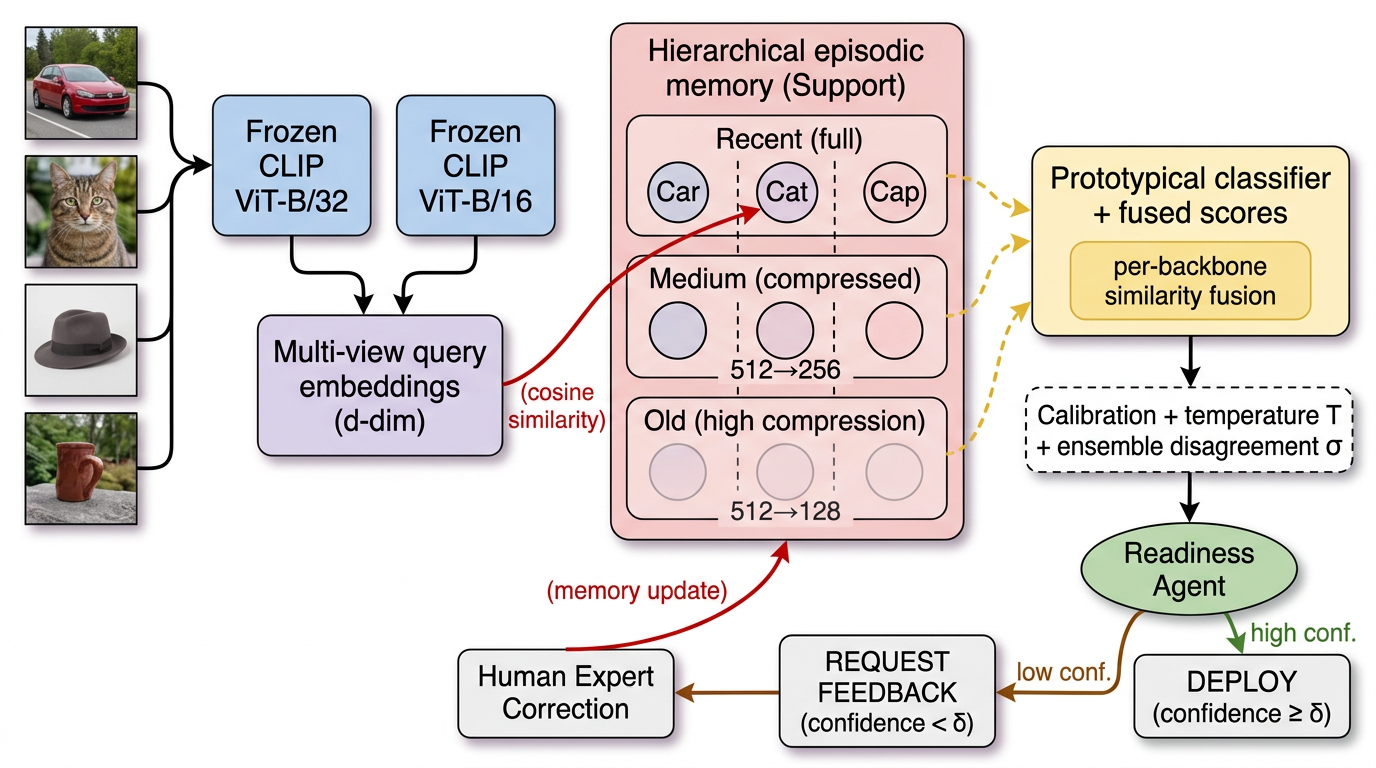
\includegraphics[width=\linewidth]{calm-v2.png}
\end{center}
\captionof{figure}{\textbf{CALM-v2 architecture and decision flow (schematic).} Each query passes through frozen CLIP ViT-B/32 and ViT-B/16 in parallel; their representations are summarized as multi-view query embeddings ($d$-dim). In the full model, class scores $\mathbf{s}^{(v)}$ are formed per backbone and fused into $\bar{\mathbf{s}}$ (Sec.~\ref{sec:method}); the figure collapses this to a single cosine-similarity arrow from the query embedding to prototypes in hierarchical episodic memory \emph{(Support)}, with recent (full), medium-compressed ($512\!\rightarrow\!256$), and old ($512\!\rightarrow\!128$) tiers and column-aligned exemplars. Dashed links from all tiers feed the prototypical classifier with fused scores; temperature~$T$ and ensemble disagreement~$\sigma$ precede the readiness agent, which \emph{deploys} if confidence $\geq\delta$ or \emph{requests feedback} if confidence $<\delta$. Expert labels update episodic memory via \emph{(memory update)} while encoders remain frozen.}
\label{fig:v2_pipeline}

\FloatBarrier
\section{Experiments}\label{sec:experiments}

\subsection{Setup}\label{sec:exp-setup}
\paragraph{Datasets and protocols.}
We evaluate on ImageNet-1k~\citep{deng2009imagenet} using the following protocols for all CALM variants: \textbf{few-shot} episodic learning with 5-way 5-shot sampling, 15 query images per class, and 600 episodes; \textbf{continual} learning with 10 sequential tasks (100 classes per task) and a 5-shot episodic memory budget per class.

\paragraph{Compared systems.}
We report \textbf{CALM-v1} (single CLIP ViT-B/32, flat memory), \textbf{CALM-v2 (ensemble)} (ViT-B/32 and ViT-B/16 with fused confidence and hierarchical memory), and, where noted, a \textbf{CALM-v2 single-backbone ablation} that keeps hierarchical memory but restricts scoring to one encoder for representation-consistent comparisons.

\paragraph{Metrics.}
Few-shot performance is mean accuracy across episodes (95\% confidence intervals for v2 where repeated seeds are available). Continual performance includes average accuracy after all tasks and backward transfer (BWT).

\subsection{Results: comparison to standard baselines}\label{sec:results-baselines}
We situate CALM-v1 and CALM-v2 next to widely cited reference numbers on the same ImageNet splits described above. The comparison is intentionally heterogeneous: backbones, training budgets, and whether parameters are updated differ across rows, so we focus on whether CALM variants behave plausibly relative to frozen-feature and classical continual baselines, rather than on declaring a universal ranking.

\paragraph{Few-shot classification (5-way 5-shot).}
Table~\ref{tab:fewshot_baselines} uses the standard episodic benchmark on ImageNet-1k~\citep{deng2009imagenet}: 600 episodes, five classes per episode, five labeled supports per class, and fifteen queries per class. We include Prototypical Networks~\citep{snell2017proto} with a ResNet-12 backbone trained end-to-end on episodic meta-learning (classic meta-learning reference); CLIP zero-shot with ViT-B/32~\citep{radford2021clip} (no task-specific support set beyond text prompts); and Tip-Adapter~\citep{zhang2022tipadapter}, a training-free cache-style adapter on top of CLIP that is a strong modern comparator for non-fine-tuned VLM adaptation. CALM-v1 and CALM-v2 rows use the same episode generator and metric (mean accuracy; for v2 we additionally report a 95\% confidence interval from repeated seeds where applicable).

\begin{table}[t]
\caption{Few-shot ImageNet (5-way 5-shot) comparison against prior methods.}
\label{tab:fewshot_baselines}
\centering
\begin{tabular}{lc}
\toprule
Method & Accuracy (\%) \\
\midrule
Prototypical Net (ResNet-12) & 77.5 \\
CLIP zero-shot (ViT-B/32) & 85.4 \\
Tip-Adapter (ViT-B/32) & 89.8 \\
\midrule
CALM-v1 & 96.88 \\
CALM-v2 (ensemble, T=1.0) & 96.16 $\pm$ 0.32 \\
CALM-v2 (ensemble, T=0.7) & 95.94 $\pm$ 0.33 \\
\bottomrule
\end{tabular}
\end{table}

CALM-v1 reaches $96.88\%$ accuracy, which is substantially higher than the listed CLIP zero-shot ($85.4\%$) and Tip-Adapter ($89.8\%$) entries under this protocol. CALM-v2 (ensemble) remains higher than those same CLIP-centric baselines at $96.16\% \pm 0.32\%$ (temperature $T=1.0$) and $95.94\% \pm 0.33\%$ ($T=0.7$), suggesting that the additional machinery in v2 does not remove the gains from episodic prototypes in our setting, while modestly lowering the point estimate relative to v1.

\paragraph{Continual learning (10 tasks, 100 classes per task).}
Table~\ref{tab:continual_baselines} reports average accuracy after all tasks and BWT on the same 10-task split. Baselines include a fine-tuning reference (severe forgetting in this table), iCaRL~\citep{rebuffi2017icarl}, and DualPrompt~\citep{wang2022dualprompt}. CALM variants keep the CLIP trunk frozen and rely on episodic memory, which is a different operating point than prompt-based continual learners that adapt internal representations.

\begin{table}[t]
\caption{Continual ImageNet (10 tasks) comparison against prior methods.}
\label{tab:continual_baselines}
\centering
\begin{tabular}{lcc}
\toprule
Method & Avg. Acc. (\%) & BWT (\%) \\
\midrule
Fine-tuning & 25.0 & -65.0 \\
iCaRL & 72.0 & -11.0 \\
DualPrompt & 88.0 & -1.2 \\
\midrule
CALM-v1 & 59.61 & -5.52 \\
CALM-v2 (ensemble, T=1.0) & 55.16 & -5.97 \\
CALM-v2 (ensemble, T=0.7) & 54.59 & -6.03 \\
\bottomrule
\end{tabular}
\end{table}

Among the listed continual baselines, DualPrompt attains the highest average accuracy ($88.0\%$) and the least negative BWT ($-1.2\%$), consistent with its prompt-based continual-learning objective. CALM-v1 attains $59.61\%$ average accuracy with BWT $-5.52\%$, which is far more stable than the fine-tuning reference ($-65.0\%$ BWT) and closer to iCaRL-level forgetting behavior than to catastrophic collapse, despite using a frozen VLM. CALM-v2 (ensemble) shows a modest reduction in average accuracy ($\approx\!55\%$) and somewhat more negative BWT than v1; we return to this pattern in Section~\ref{sec:discussion}.

\subsection{Results: CALM-v1 versus CALM-v2 under matched protocols}\label{sec:results-v1v2}
\begin{table}[t]
\caption{ImageNet-aligned comparison of CALM-v1 and CALM-v2 variants.}
\label{tab:main}
\centering
\begin{tabular}{lccc}
\toprule
Method & 5-way 5-shot (\%) & Avg. Acc. (\%) & BWT (\%) \\
\midrule
CALM-v1 & 96.88 & 59.61 & -5.52 \\
CALM-v2 ensemble (T=1.0) & 96.16 $\pm$ 0.32 & 55.16 & -5.97 \\
CALM-v2 ensemble (T=0.7) & 95.94 $\pm$ 0.33 & 54.59 & -6.03 \\
\bottomrule
\end{tabular}
\end{table}

Table~\ref{tab:main} places few-shot accuracy, average continual accuracy, and BWT side-by-side for CALM-v1 and the CALM-v2 ensemble settings we evaluated, using matched scripts and temperatures.

\subsection{Discussion and recommendations}\label{sec:discussion}
\paragraph{Interpretation.}
One explanation that is consistent with our implementation inspection is \textbf{embedding-space mismatch}: if support prototypes are formed primarily in one backbone space (e.g., ViT-B/32) while query scoring blends similarities from another encoder (e.g., ViT-B/16) without aligned prototypes or projections, cosine scores need not behave like distances in a single metric space, which can erode margins. We treat this as a plausible and testable account rather than a unique root cause; compression noise and fusion hyperparameters may contribute as well.

\paragraph{Practical recommendations.}
Based on the observed behavior and engineering review of the codebase, we suggest:
\begin{enumerate}
    \item Prefer a \textbf{single-space classification path} when possible: score queries and supports in the same encoder unless per-backbone prototypes are maintained.
    \item \textbf{Pretrain compression modules} on in-domain (e.g., ImageNet) embeddings before long continual runs to limit reconstruction bias.
    \item If multi-encoder fusion is kept, \textbf{tune weights and temperature} on held-out validation episodes rather than relying on defaults.
    \item Consider \textbf{separating roles}: use ensemble disagreement mainly for readiness while keeping the classifier in a representation-consistent subspace.
\end{enumerate}

\begin{center}
\begin{tikzpicture}[x=1cm,y=1cm]
\draw[->] (0,0) -- (6.5,0) node[right] {few-shot accuracy (\%)};
\draw[->] (0,0) -- (0,4.0) node[above] {continual avg. acc. (\%)};
\node[circle,fill=blue!70,inner sep=2.8pt,label=below:{\scriptsize CALM-v1}] at (5.8,3.1) {};
\node[circle,fill=red!70,inner sep=2.8pt,label=below:{\scriptsize v2 ensemble}] at (5.4,2.5) {};
\node[circle,fill=green!60!black,inner sep=2.8pt,label=above:{\scriptsize target region}] at (5.7,3.0) {};
\draw[dashed] (5.8,0) -- (5.8,3.1);
\draw[dashed] (0,3.1) -- (5.8,3.1);
\draw[dashed] (5.4,0) -- (5.4,2.5);
\draw[dashed] (0,2.5) -- (5.4,2.5);
\end{tikzpicture}
\end{center}
\captionof{figure}{\textbf{Qualitative view of measured ImageNet trade-offs (cf.\ Table~\ref{tab:main}).} CALM-v1 (blue) achieves higher few-shot accuracy and continual average accuracy than the CALM-v2 ensemble (red) in our reported runs. Dashed guides highlight the horizontal and vertical separation between the two operating points. The green marker sketches a desirable region that would combine v1-like task metrics with v2's motivation for richer confidence and scalable memory; closing that gap is an engineering target (e.g., consistent single-space scoring and tuned fusion), not something this plot claims to achieve.}
\label{fig:tradeoff}

\subsection{Limitations}\label{sec:limitations}
Our study prioritizes protocol alignment across versions, but continual learning results would benefit from broader repeated-seed reporting; the CALM-v2 single-backbone ablation is implemented, yet full aggregate statistics are still being consolidated. Readiness-agent end-to-end deployment metrics for CALM-v2 on ImageNet are not fully unified in this draft, so we limit claims to the few-shot and continual core-engine numbers shown above. Finally, all conclusions are conditional on ImageNet-style natural images and public CLIP checkpoints; other domains may exhibit different calibration and memory effects.

\section{Broader Impact}
Reliable adaptation of visual systems may positively impact settings where frequent retraining is infeasible (e.g., low-resource medical triage support and assistive monitoring). Potential risks include over-trust in autonomous decisions and dataset-specific biases from pretrained backbones. CALM-style readiness gating, uncertainty thresholds, and human feedback pathways are intended as mitigations, but careful deployment governance remains essential.

\section{Conclusion}
We presented CALM-v1 and CALM-v2 as a single non-parametric adaptation story built on frozen VLMs, episodic prototypes, and readiness-aware deployment. Under the ImageNet protocols we used, CALM-v1 yields favorable few-shot accuracy relative to several listed CLIP-centric baselines, and CALM-v2 remains in a similar accuracy range while introducing ensemble confidence and hierarchical memory intended for deployment constraints. The v2 configuration we evaluated shows somewhat lower average continual accuracy than v1 in our tables; we outlined a representation-consistency narrative and engineering steps that may help narrow that gap in future work. We hope this first unified account of both variants, together with benchmarks and limitations, supports further refinement before submission.

\begin{ack}
This work uses publicly available models and datasets, including CLIP and ImageNet. The project follows the NeurIPS guidelines for reproducibility and responsible reporting to the extent possible in an academic setting with limited compute resources.
\end{ack}

\nocite{he2024peftsurvey,lester2021prompttuning,houlsby2019adapters,hu2022lora,wang2024vladapter,chen2024trainclip,wang2024llmclsurvey,wang2022l2p,lomonaco2024continualreview,smith2024cops,chen2024conformalvlm,liu2024oodllm,zhang2024hallucinationvlm,zhang2024humanloop,martinez2024hri,thompson2024calibration,davis2024vlmreview,krizhevsky2009cifar,coates2011stl10,xiao2017fashionmnist}

\bibliographystyle{plainnat}
\bibliography{references}

\appendix
\newpage
\section*{NeurIPS Paper Checklist}


\begin{enumerate}

\item {\bf Claims}
    \item[] Question: Do the main claims made in the abstract and introduction accurately reflect the paper's contributions and scope?
    \item[] Answer: \answerYes{}
    \item[] Justification: The abstract and introduction describe the contribution scope as an ImageNet-aligned CALM-v1 vs CALM-v2 comparison and analysis of architectural trade-offs (Sections 1 and 4).
    \item[] Guidelines:
    \begin{itemize}
        \item The answer \answerNA{} means that the abstract and introduction do not include the claims made in the paper.
        \item The abstract and/or introduction should clearly state the claims made, including the contributions made in the paper and important assumptions and limitations. A \answerNo{} or \answerNA{} answer to this question will not be perceived well by the reviewers. 
        \item The claims made should match theoretical and experimental results, and reflect how much the results can be expected to generalize to other settings. 
        \item It is fine to include aspirational goals as motivation as long as it is clear that these goals are not attained by the paper. 
    \end{itemize}

\item {\bf Limitations}
    \item[] Question: Does the paper discuss the limitations of the work performed by the authors?
    \item[] Answer: \answerYes{}
    \item[] Justification: Limitations are discussed in a dedicated subsection (Section 4.5) covering seed count, pending readiness-agent consolidation, and scope boundaries.
    \item[] Guidelines:
    \begin{itemize}
        \item The answer \answerNA{} means that the paper has no limitation while the answer \answerNo{} means that the paper has limitations, but those are not discussed in the paper. 
        \item The authors are encouraged to create a separate ``Limitations'' section in their paper.
        \item The paper should point out any strong assumptions and how robust the results are to violations of these assumptions (e.g., independence assumptions, noiseless settings, model well-specification, asymptotic approximations only holding locally). The authors should reflect on how these assumptions might be violated in practice and what the implications would be.
        \item The authors should reflect on the scope of the claims made, e.g., if the approach was only tested on a few datasets or with a few runs. In general, empirical results often depend on implicit assumptions, which should be articulated.
        \item The authors should reflect on the factors that influence the performance of the approach. For example, a facial recognition algorithm may perform poorly when image resolution is low or images are taken in low lighting. Or a speech-to-text system might not be used reliably to provide closed captions for online lectures because it fails to handle technical jargon.
        \item The authors should discuss the computational efficiency of the proposed algorithms and how they scale with dataset size.
        \item If applicable, the authors should discuss possible limitations of their approach to address problems of privacy and fairness.
        \item While the authors might fear that complete honesty about limitations might be used by reviewers as grounds for rejection, a worse outcome might be that reviewers discover limitations that aren't acknowledged in the paper. The authors should use their best judgment and recognize that individual actions in favor of transparency play an important role in developing norms that preserve the integrity of the community. Reviewers will be specifically instructed to not penalize honesty concerning limitations.
    \end{itemize}

\item {\bf Theory assumptions and proofs}
    \item[] Question: For each theoretical result, does the paper provide the full set of assumptions and a complete (and correct) proof?
    \item[] Answer: \answerNA{}
    \item[] Justification: The paper is empirical/systems-oriented and does not claim new formal theorems requiring proofs.
    \item[] Guidelines:
    \begin{itemize}
        \item The answer \answerNA{} means that the paper does not include theoretical results. 
        \item All the theorems, formulas, and proofs in the paper should be numbered and cross-referenced.
        \item All assumptions should be clearly stated or referenced in the statement of any theorems.
        \item The proofs can either appear in the main paper or the supplemental material, but if they appear in the supplemental material, the authors are encouraged to provide a short proof sketch to provide intuition. 
        \item Inversely, any informal proof provided in the core of the paper should be complemented by formal proofs provided in appendix or supplemental material.
        \item Theorems and Lemmas that the proof relies upon should be properly referenced. 
    \end{itemize}

    \item {\bf Experimental result reproducibility}
    \item[] Question: Does the paper fully disclose all the information needed to reproduce the main experimental results of the paper to the extent that it affects the main claims and/or conclusions of the paper (regardless of whether the code and data are provided or not)?
    \item[] Answer: \answerYes{}
    \item[] Justification: We provide explicit dataset and protocol settings for few-shot and continual evaluations in Sec.~\ref{sec:exp-setup} and Method (Sec.~\ref{sec:method}), consistent with the evaluation scripts in the anonymized codebase.
    \item[] Guidelines:
    \begin{itemize}
        \item The answer \answerNA{} means that the paper does not include experiments.
        \item If the paper includes experiments, a \answerNo{} answer to this question will not be perceived well by the reviewers: Making the paper reproducible is important, regardless of whether the code and data are provided or not.
        \item If the contribution is a dataset and\slash or model, the authors should describe the steps taken to make their results reproducible or verifiable. 
        \item Depending on the contribution, reproducibility can be accomplished in various ways. For example, if the contribution is a novel architecture, describing the architecture fully might suffice, or if the contribution is a specific model and empirical evaluation, it may be necessary to either make it possible for others to replicate the model with the same dataset, or provide access to the model. In general. releasing code and data is often one good way to accomplish this, but reproducibility can also be provided via detailed instructions for how to replicate the results, access to a hosted model (e.g., in the case of a large language model), releasing of a model checkpoint, or other means that are appropriate to the research performed.
        \item While NeurIPS does not require releasing code, the conference does require all submissions to provide some reasonable avenue for reproducibility, which may depend on the nature of the contribution. For example
        \begin{enumerate}
            \item If the contribution is primarily a new algorithm, the paper should make it clear how to reproduce that algorithm.
            \item If the contribution is primarily a new model architecture, the paper should describe the architecture clearly and fully.
            \item If the contribution is a new model (e.g., a large language model), then there should either be a way to access this model for reproducing the results or a way to reproduce the model (e.g., with an open-source dataset or instructions for how to construct the dataset).
            \item We recognize that reproducibility may be tricky in some cases, in which case authors are welcome to describe the particular way they provide for reproducibility. In the case of closed-source models, it may be that access to the model is limited in some way (e.g., to registered users), but it should be possible for other researchers to have some path to reproducing or verifying the results.
        \end{enumerate}
    \end{itemize}


\item {\bf Open access to data and code}
    \item[] Question: Does the paper provide open access to the data and code, with sufficient instructions to faithfully reproduce the main experimental results, as described in supplemental material?
    \item[] Answer: \answerNo{}
    \item[] Justification: ImageNet redistribution constraints prevent open data release; however, code paths are documented in the repository to allow replication for authorized users with dataset access, alongside protocol detail in the main text.
    \item[] Guidelines:
    \begin{itemize}
        \item The answer \answerNA{} means that paper does not include experiments requiring code.
        \item Please see the NeurIPS code and data submission guidelines (\url{https://neurips.cc/public/guides/CodeSubmissionPolicy}) for more details.
        \item While we encourage the release of code and data, we understand that this might not be possible, so \answerNo{} is an acceptable answer. Papers cannot be rejected simply for not including code, unless this is central to the contribution (e.g., for a new open-source benchmark).
        \item The instructions should contain the exact command and environment needed to run to reproduce the results. See the NeurIPS code and data submission guidelines (\url{https://neurips.cc/public/guides/CodeSubmissionPolicy}) for more details.
        \item The authors should provide instructions on data access and preparation, including how to access the raw data, preprocessed data, intermediate data, and generated data, etc.
        \item The authors should provide scripts to reproduce all experimental results for the new proposed method and baselines. If only a subset of experiments are reproducible, they should state which ones are omitted from the script and why.
        \item At submission time, to preserve anonymity, the authors should release anonymized versions (if applicable).
        \item Providing as much information as possible in supplemental material (appended to the paper) is recommended, but including URLs to data and code is permitted.
    \end{itemize}


\item {\bf Experimental setting/details}
    \item[] Question: Does the paper specify all the training and test details (e.g., data splits, hyperparameters, how they were chosen, type of optimizer) necessary to understand the results?
    \item[] Answer: \answerYes{}
    \item[] Justification: The manuscript specifies splits, episode/task setup, temperatures, memory shots, and compared variants needed to interpret the results.
    \item[] Guidelines:
    \begin{itemize}
        \item The answer \answerNA{} means that the paper does not include experiments.
        \item The experimental setting should be presented in the core of the paper to a level of detail that is necessary to appreciate the results and make sense of them.
        \item The full details can be provided either with the code, in appendix, or as supplemental material.
    \end{itemize}

\item {\bf Experiment statistical significance}
    \item[] Question: Does the paper report error bars suitably and correctly defined or other appropriate information about the statistical significance of the experiments?
    \item[] Answer: \answerNo{}
    \item[] Justification: We report 95\% confidence intervals for few-shot episodes, but continual results are currently single-run and do not yet include multi-seed variance.
    \item[] Guidelines:
    \begin{itemize}
        \item The answer \answerNA{} means that the paper does not include experiments.
        \item The authors should answer \answerYes{} if the results are accompanied by error bars, confidence intervals, or statistical significance tests, at least for the experiments that support the main claims of the paper.
        \item The factors of variability that the error bars are capturing should be clearly stated (for example, train/test split, initialization, random drawing of some parameter, or overall run with given experimental conditions).
        \item The method for calculating the error bars should be explained (closed form formula, call to a library function, bootstrap, etc.)
        \item The assumptions made should be given (e.g., Normally distributed errors).
        \item It should be clear whether the error bar is the standard deviation or the standard error of the mean.
        \item It is OK to report 1-sigma error bars, but one should state it. The authors should preferably report a 2-sigma error bar than state that they have a 96\% CI, if the hypothesis of Normality of errors is not verified.
        \item For asymmetric distributions, the authors should be careful not to show in tables or figures symmetric error bars that would yield results that are out of range (e.g., negative error rates).
        \item If error bars are reported in tables or plots, the authors should explain in the text how they were calculated and reference the corresponding figures or tables in the text.
    \end{itemize}

\item {\bf Experiments compute resources}
    \item[] Question: For each experiment, does the paper provide sufficient information on the computer resources (type of compute workers, memory, time of execution) needed to reproduce the experiments?
    \item[] Answer: \answerNo{}
    \item[] Justification: We report practical execution commands and settings, but a full resource accounting table (GPU model, memory, per-run time) is not yet complete.
    \item[] Guidelines:
    \begin{itemize}
        \item The answer \answerNA{} means that the paper does not include experiments.
        \item The paper should indicate the type of compute workers CPU or GPU, internal cluster, or cloud provider, including relevant memory and storage.
        \item The paper should provide the amount of compute required for each of the individual experimental runs as well as estimate the total compute. 
        \item The paper should disclose whether the full research project required more compute than the experiments reported in the paper (e.g., preliminary or failed experiments that didn't make it into the paper). 
    \end{itemize}
    
\item {\bf Code of ethics}
    \item[] Question: Does the research conducted in the paper conform, in every respect, with the NeurIPS Code of Ethics \url{https://neurips.cc/public/EthicsGuidelines}?
    \item[] Answer: \answerYes{}
    \item[] Justification: The work uses standard academic benchmarks and reports limitations and deployment cautions; no human-subject interventions were conducted.
    \item[] Guidelines:
    \begin{itemize}
        \item The answer \answerNA{} means that the authors have not reviewed the NeurIPS Code of Ethics.
        \item If the authors answer \answerNo, they should explain the special circumstances that require a deviation from the Code of Ethics.
        \item The authors should make sure to preserve anonymity (e.g., if there is a special consideration due to laws or regulations in their jurisdiction).
    \end{itemize}


\item {\bf Broader impacts}
    \item[] Question: Does the paper discuss both potential positive societal impacts and negative societal impacts of the work performed?
    \item[] Answer: \answerYes{}
    \item[] Justification: We discuss positive use cases and possible risks (over-trust, bias, misuse) together with mitigation perspective in the broader impact section.
    \item[] Guidelines:
    \begin{itemize}
        \item The answer \answerNA{} means that there is no societal impact of the work performed.
        \item If the authors answer \answerNA{} or \answerNo, they should explain why their work has no societal impact or why the paper does not address societal impact.
        \item Examples of negative societal impacts include potential malicious or unintended uses (e.g., disinformation, generating fake profiles, surveillance), fairness considerations (e.g., deployment of technologies that could make decisions that unfairly impact specific groups), privacy considerations, and security considerations.
        \item The conference expects that many papers will be foundational research and not tied to particular applications, let alone deployments. However, if there is a direct path to any negative applications, the authors should point it out. For example, it is legitimate to point out that an improvement in the quality of generative models could be used to generate Deepfakes for disinformation. On the other hand, it is not needed to point out that a generic algorithm for optimizing neural networks could enable people to train models that generate Deepfakes faster.
        \item The authors should consider possible harms that could arise when the technology is being used as intended and functioning correctly, harms that could arise when the technology is being used as intended but gives incorrect results, and harms following from (intentional or unintentional) misuse of the technology.
        \item If there are negative societal impacts, the authors could also discuss possible mitigation strategies (e.g., gated release of models, providing defenses in addition to attacks, mechanisms for monitoring misuse, mechanisms to monitor how a system learns from feedback over time, improving the efficiency and accessibility of ML).
    \end{itemize}
    
\item {\bf Safeguards}
    \item[] Question: Does the paper describe safeguards that have been put in place for responsible release of data or models that have a high risk for misuse (e.g., pre-trained language models, image generators, or scraped datasets)?
    \item[] Answer: \answerNA{}
    \item[] Justification: The paper does not release a new high-risk generative model or scraped dataset; it evaluates adaptation methods on established benchmarks.
    \item[] Guidelines:
    \begin{itemize}
        \item The answer \answerNA{} means that the paper poses no such risks.
        \item Released models that have a high risk for misuse or dual-use should be released with necessary safeguards to allow for controlled use of the model, for example by requiring that users adhere to usage guidelines or restrictions to access the model or implementing safety filters. 
        \item Datasets that have been scraped from the Internet could pose safety risks. The authors should describe how they avoided releasing unsafe images.
        \item We recognize that providing effective safeguards is challenging, and many papers do not require this, but we encourage authors to take this into account and make a best faith effort.
    \end{itemize}

\item {\bf Licenses for existing assets}
    \item[] Question: Are the creators or original owners of assets (e.g., code, data, models), used in the paper, properly credited and are the license and terms of use explicitly mentioned and properly respected?
    \item[] Answer: \answerYes{}
    \item[] Justification: The manuscript cites CLIP and benchmark datasets; usage follows public research access norms and associated terms for those assets.
    \item[] Guidelines:
    \begin{itemize}
        \item The answer \answerNA{} means that the paper does not use existing assets.
        \item The authors should cite the original paper that produced the code package or dataset.
        \item The authors should state which version of the asset is used and, if possible, include a URL.
        \item The name of the license (e.g., CC-BY 4.0) should be included for each asset.
        \item For scraped data from a particular source (e.g., website), the copyright and terms of service of that source should be provided.
        \item If assets are released, the license, copyright information, and terms of use in the package should be provided. For popular datasets, \url{paperswithcode.com/datasets} has curated licenses for some datasets. Their licensing guide can help determine the license of a dataset.
        \item For existing datasets that are re-packaged, both the original license and the license of the derived asset (if it has changed) should be provided.
        \item If this information is not available online, the authors are encouraged to reach out to the asset's creators.
    \end{itemize}

\item {\bf New assets}
    \item[] Question: Are new assets introduced in the paper well documented and is the documentation provided alongside the assets?
    \item[] Answer: \answerYes{}
    \item[] Justification: New evaluation scripts and protocols are documented with commands and folder-level README instructions.
    \item[] Guidelines:
    \begin{itemize}
        \item The answer \answerNA{} means that the paper does not release new assets.
        \item Researchers should communicate the details of the dataset\slash code\slash model as part of their submissions via structured templates. This includes details about training, license, limitations, etc. 
        \item The paper should discuss whether and how consent was obtained from people whose asset is used.
        \item At submission time, remember to anonymize your assets (if applicable). You can either create an anonymized URL or include an anonymized zip file.
    \end{itemize}

\item {\bf Crowdsourcing and research with human subjects}
    \item[] Question: For crowdsourcing experiments and research with human subjects, does the paper include the full text of instructions given to participants and screenshots, if applicable, as well as details about compensation (if any)? 
    \item[] Answer: \answerNA{}
    \item[] Justification: The work does not involve crowdsourcing or human-subject experiments.
    \item[] Guidelines:
    \begin{itemize}
        \item The answer \answerNA{} means that the paper does not involve crowdsourcing nor research with human subjects.
        \item Including this information in the supplemental material is fine, but if the main contribution of the paper involves human subjects, then as much detail as possible should be included in the main paper. 
        \item According to the NeurIPS Code of Ethics, workers involved in data collection, curation, or other labor should be paid at least the minimum wage in the country of the data collector. 
    \end{itemize}

\item {\bf Institutional review board (IRB) approvals or equivalent for research with human subjects}
    \item[] Question: Does the paper describe potential risks incurred by study participants, whether such risks were disclosed to the subjects, and whether Institutional Review Board (IRB) approvals (or an equivalent approval/review based on the requirements of your country or institution) were obtained?
    \item[] Answer: \answerNA{}
    \item[] Justification: No human-subject participation or intervention is part of the reported experiments.
    \item[] Guidelines:
    \begin{itemize}
        \item The answer \answerNA{} means that the paper does not involve crowdsourcing nor research with human subjects.
        \item Depending on the country in which research is conducted, IRB approval (or equivalent) may be required for any human subjects research. If you obtained IRB approval, you should clearly state this in the paper. 
        \item We recognize that the procedures for this may vary significantly between institutions and locations, and we expect authors to adhere to the NeurIPS Code of Ethics and the guidelines for their institution. 
        \item For initial submissions, do not include any information that would break anonymity (if applicable), such as the institution conducting the review.
    \end{itemize}

\item {\bf Declaration of LLM usage}
    \item[] Question: Does the paper describe the usage of LLMs if it is an important, original, or non-standard component of the core methods in this research? Note that if the LLM is used only for writing, editing, or formatting purposes and does \emph{not} impact the core methodology, scientific rigor, or originality of the research, declaration is not required.
    %this research? 
    \item[] Answer: \answerNA{}
    \item[] Justification: LLMs are not a core methodological component of the proposed adaptation framework or evaluation pipeline.
    \item[] Guidelines:
    \begin{itemize}
        \item The answer \answerNA{} means that the core method development in this research does not involve LLMs as any important, original, or non-standard components.
        \item Please refer to our LLM policy in the NeurIPS handbook for what should or should not be described.
    \end{itemize}

\end{enumerate}
\end{document}